% This work is licensed under the Creative Commons
% Attribution-NonCommercial-ShareAlike 4.0 International License. To view a copy
% of this license, visit http://creativecommons.org/licenses/by-nc-sa/4.0/ or
% send a letter to Creative Commons, PO Box 1866, Mountain View, CA 94042, USA.

\section{Parameterschätzung in linearen Modellen}

\begin{definition}\label{def3.1}\
	\begin{enumerate}[label=(\arabic*)]
		\item Sei $Z:=\big(Z_{i,j}\big)_{\begin{subarray}{c}
			1\leq i\leq m\\
			1\leq j\leq n
		\end{subarray}}\in M(m\times n)$
		mit integrierbaren Komponenten $Z_{i,j}$, welche reelle Zufallsvariablen sind.
		Dann: \label{item:def3.1(1)}
		\begin{align*}
			\E[Z]:=\Big(\E\big[Z_{i,j}\big]\Big)_{\begin{subarray}{c}
			1\leq i\leq m\\
			1\leq j\leq n
		\end{subarray}}
		\end{align*}
		Speziell für 
		\begin{align*}
			Z=\big(Z_1,\ldots,Z_m\big)'
		\end{align*}
		ist 
		\begin{align*}
			\E[Z]=\begin{pmatrix}
				\E\big[Z_1\big]\\
				\vdots\\
				\E\big[Z_n\big]
			\end{pmatrix}=\Big(\E\big[Z_1\big],\ldots,\E\big[Z_n\big]\Big)'
		\end{align*}
		\item Seien
		\begin{align*}
			Z=\big(Z_1,\ldots,Z_m\big)',\qquad
			Y=\big(Y_1,\ldots,Y_n\big)'.
		\end{align*}		 
		Dann, falls existent
		\begin{align*}
			\Cov(Y,Z)&:=\E\Big(\big(Y-\E[Y]\big)\mal\big(Z-\E[Z]\big)'\Big)\\
			\overset{\ref{item:def3.1(1)}}&{~=}
			\klammern[\bigg]{\E\Big[\big(Y_i-\E[Y_i]\big)\mal\big(Z_j-\E[Z_j]\big)\Big]}_{\begin{subarray}{c}
			1\leq i\leq m\\
			1\leq j\leq n
		\end{subarray}}\\
		&~=\Big(\Cov(Y_i,Z_j)\Big)_{\begin{subarray}{c}
			1\leq i\leq m\\
			1\leq j\leq n
		\end{subarray}}
		\end{align*}
		Speziell ist\index{Kovarianzmatrix}
		\begin{align*}
			\Var(Y):=\Cov(Y,Y)=\Big(\Cov(Y_i,Y_j)\Big)_{\begin{subarray}{c}
			1\leq i\leq m\\
			1\leq j\leq n
		\end{subarray}}\in M(n\times n)
		\end{align*}
		die \define{Kovarianzmatrix} von $Y$.
	\end{enumerate}
\end{definition}

\begin{satz}\label{satz3.2}
	Seien $Y$ und $Z$ Zufallsvektoren in $\R^n$ bzw. $\R^m$, $A\in M(m\times n)$, $b\in\R^m$ beide deterministisch.
	Dann gilt:
	\begin{enumerate}[label=(\arabic*)]
		\item $\begin{aligned}
			\E\big[A\mal Y+Z\big]=A\mal\E[Y]+\E[Z]
		\end{aligned}\qquad$ ($\E$ ist linear)
		\label{item:satz3.2(1)}
		\item $\begin{aligned}
			\Var\big(A\mal Y+b\big)=A\mal\Var(Y)\mal A'
		\end{aligned}$
		\label{item:satz3.2(2)}
	\end{enumerate}
\end{satz}

\begin{proof}
	Nachrechnen! (Zur Übung, folgt aus Matrixmultiplikation + den Eigenschaften im reellen Fall)
	%\betone{Zeige \ref{item:satz3.2(1)}:}\\
	
	%\betone{Zeige \ref{item:satz3.2(2)}:}\\
\end{proof}

Wir betrachten jetzt das lineare Modell (vergleiche \eqref{eq:1.2}) mit 
\begin{align}\label{eq:3.1}\tag{3.1}
	Y&=X\mal\beta+\varepsilon\\
	\E[\varepsilon]&=0\label{eq:3.2}\tag{3.2}\\
	\Var(\varepsilon)&=\sigma^2\mal I_n\mit\sigma^2>0\label{eq:3.3}\tag{3.3}\\
	n&\geq p\label{eq:3.4}\tag{3.4}
\end{align}
Beachte ($\varepsilon=\big(\varepsilon_1,\ldots,\varepsilon_n\big)'$):
\begin{align*}
	\eqref{eq:3.3}&\iff\Cov(\varepsilon_i,\varepsilon_j)=\sigma^2\mal\delta_{i,j}
	&&\forall i,j\\
	&\iff\Cov\big(\varepsilon_i,\varepsilon_j\big)=0
	&&\forall i\neq j\und\Var(\varepsilon_i)=\sigma^2
\end{align*}
Also gilt: $\varepsilon_1,\ldots,\varepsilon_n$ iid $\implies\eqref{eq:3.3}$\\
($p$ ist die Anzahl der Modellparameter)
\begin{align*}
	\eqref{eq:3.1}\iff Y_i=\sum\limits_{j=1}^p X_{i,j}\mal\beta_j+\varepsilon_i\quad\forall i
\end{align*}

\subsection{Minimum-Quadrat-Schätzer}

Ziel: Schätzung von $\beta$.
Idee nach Gauß und Legendre: 
\define{Methode der kleinsten Quadrate}, nämlich:
Minimierung der \define{Fehlerquadratsumme}
\index{Fehlerquadratsumme}\index{Methode der kleinsten Quadrate}
\begin{align*}
	\sum\limits_{i=1}^n\varepsilon_i^2
	\overset{\Def}&{=}
	\norm{\varepsilon}^2
	\overset{\eqref{eq:3.1}}{=}
	\norm{Y-X\mal\beta}^2,
\end{align*}
d.h. finde $\hat{\beta}$ mit
\begin{align*}
	&\hspace{11.5mm}\norm{Y-X\mal\hat{\beta}}^2\leq\norm{Y-X\mal\beta}^2&&\forall\beta\in\R^p\\
	&\iff
	\norm{Y-X\mal\hat{\beta}}\leq\norm{Y-X\mal\beta}&&\forall\beta\in\R^p\\
	&\iff\hat{\beta}(\omega)\in\argmin\limits_{\beta\in\R^p}\norm{Y(\omega)-X\mal\beta}
\end{align*}
Die Lösung ist bekannt.
Es gilt

\begin{satz}\label{satz3.3}
	Es gelten \eqref{eq:3.1} und \eqref{eq:3.4}.
	Dann gilt:
	\begin{enumerate}[label=(\arabic*)]
		\item Die Minimalstelle $\hat{\beta}$ existiert und erfüllt die \define{Normalgleichung} \label{item:satz3.3(1)}
		\index{Normalgleichung}
		\begin{align}\label{eq:satz3.3Stern}\tag{$*$}
			X'\mal X\mal\hat{\beta}=X'\mal Y
		\end{align}
		und umgekehrt ist jede Lösung von \eqref{eq:satz3.3Stern} eine Minimalstelle.\\
		Bezeichnet $L:=\Bild(X)$, so gilt:
		\begin{align*}
			P_L(Y)=X\mal\hat{\beta}
		\end{align*}
		\item Falls $\Rg(X)=p$ (also Vollrang), so gilt:\label{item:satz3.3(2)}
		\begin{align*}
			\hat{\beta}&=\big(X'\mal X)^{-1}\mal X'\mal Y
			\qquad\und\qquad
			P_L=X\mal\big(X'\mal X\big)^{-1}\mal X'
		\end{align*}
		Der Schätzer $\hat{\beta}$ heißt \define{Minimum-Quadrat-Schätzer (MQS) /\\ Kleinst-Quadrate-Schätzer (KQS) / least squares estimator (lse)}.
		\index{Minimum-Qudrat-Schätzer}
		\index{Kleinst-Quadrate-Schätzer}
		\index{least squares estimator|see{Minimum-Quadrat-Schätzer}}
	\end{enumerate}
\end{satz}

\begin{proof}
	Nutze Satz \ref{satz2.22} mit $A\leftrightarrow X$, $x\leftrightarrow Y(\omega)$ und $y\leftrightarrow\beta$.
\end{proof}

\begin{figure}[H]
	\begin{center}
		% This work is licensed under the Creative Commons
% Attribution-NonCommercial-ShareAlike 4.0 International License. To view a copy
% of this license, visit http://creativecommons.org/licenses/by-nc-sa/4.0/ or
% send a letter to Creative Commons, PO Box 1866, Mountain View, CA 94042, USA.



\tikzset{every picture/.style={line width=0.75pt}} %set default line width to 0.75pt        

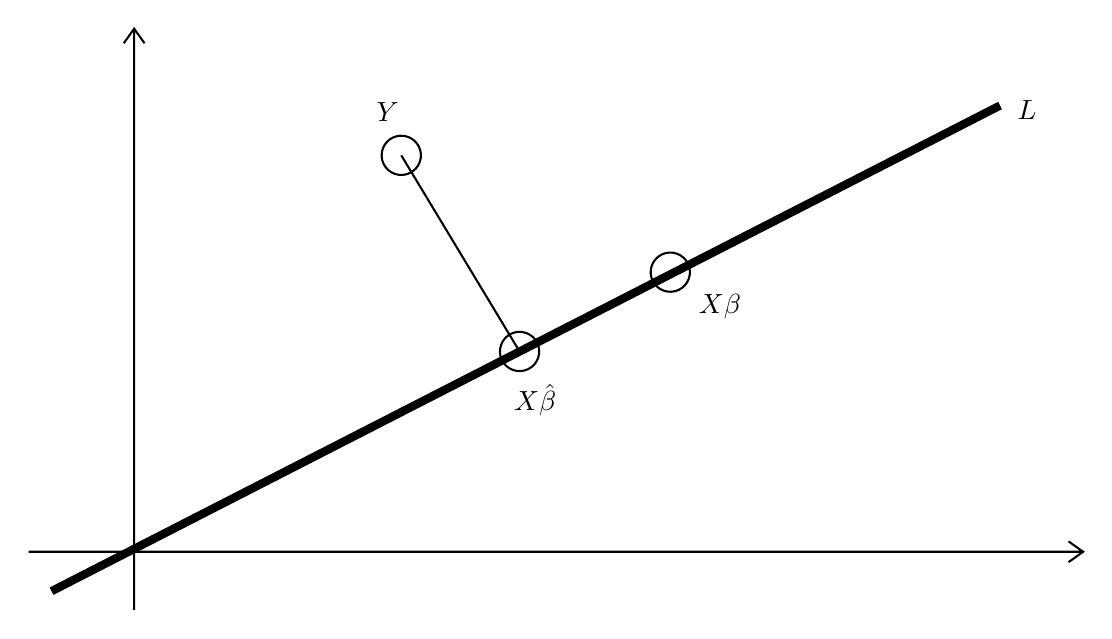
\begin{tikzpicture}[x=0.75pt,y=0.75pt,yscale=-1,xscale=1]
%uncomment if require: \path (0,300); %set diagram left start at 0, and has height of 300

%Shape: Axis 2D [id:dp7098119764904821] 
\draw  (50,256.93) -- (558,256.93)(100.8,4.93) -- (100.8,284.93) (551,251.93) -- (558,256.93) -- (551,261.93) (95.8,11.93) -- (100.8,4.93) -- (105.8,11.93)  ;
%Straight Lines [id:da9071558730776327] 
\draw [line width=3]    (61,275.93) -- (518,41.93) ;


%Straight Lines [id:da7398348018165936] 
\draw    (210,68.93) ;


%Straight Lines [id:da721943207149605] 
\draw    (229.5,65.93) -- (286.5,160.43) ;


%Shape: Circle [id:dp22369371272099947] 
\draw   (277.13,159.1) .. controls (277.87,153.92) and (282.66,150.33) .. (287.84,151.07) .. controls (293.01,151.81) and (296.61,156.6) .. (295.87,161.77) .. controls (295.13,166.94) and (290.34,170.54) .. (285.16,169.8) .. controls (279.99,169.06) and (276.39,164.27) .. (277.13,159.1) -- cycle ;
%Shape: Circle [id:dp5421173957527967] 
\draw   (349.75,120.88) .. controls (350.49,115.71) and (355.28,112.12) .. (360.45,112.86) .. controls (365.63,113.59) and (369.22,118.39) .. (368.48,123.56) .. controls (367.74,128.73) and (362.95,132.33) .. (357.78,131.59) .. controls (352.6,130.85) and (349.01,126.06) .. (349.75,120.88) -- cycle ;
%Shape: Circle [id:dp28472585647194326] 
\draw   (220.13,64.6) .. controls (220.87,59.42) and (225.66,55.83) .. (230.84,56.57) .. controls (236.01,57.31) and (239.61,62.1) .. (238.87,67.27) .. controls (238.13,72.44) and (233.34,76.04) .. (228.16,75.3) .. controls (222.99,74.56) and (219.39,69.77) .. (220.13,64.6) -- cycle ;

% Text Node
\draw (531,43.93) node  [align=left] {$L$};
% Text Node
\draw (223,44.93) node  [align=left] {$Y$};
% Text Node
\draw (294,183.93) node  [align=left] {$X\mal\hat{\beta}$};
% Text Node
\draw (383,138.93) node  [align=left] {$X\mal\beta$};


\end{tikzpicture}

		\caption{Minimum-Quadrat-Schätzer}
		\label{Abb:MinQuaSchätzer}
	\end{center}
\end{figure}

\begin{satz}\label{satz3.4}
	Angenommen es gelten \eqref{eq:3.1}, \eqref{eq:3.2}, \eqref{eq:3.3} und \eqref{eq:3.4}.
	Falls $\Rg(X)=p$, so gilt:
	\begin{align}\label{eq:3.5}\tag{3.5}
		\E\big[\hat{\beta}\big]&=\beta\qquad\forall\beta\in\R^p\\
		\Var\big(\hat{\beta}\big)&=\sigma^2\mal\big(X'\mal X\big)^{-1}\label{eq:3.6}\tag{3.6}
	\end{align}
\end{satz}

\begin{proof}
	\begin{align*}
		\E\big[\hat{\beta}\big]
		\overset{\ref{satz3.3}\ref{item:satz3.3(2)}}&{=}
		\E\Big[\underbrace{\big((X'\mal X)^{-1}\mal X'\big)}_{=:A}\mal Y\Big]\\
		\overset{\ref{satz3.2}\ref{item:satz3.2(1)}}&{=}
		\big(X'\mal X\big)^{-1}\mal X'\mal\E[Y]\\
		\overset{\eqref{eq:3.1}}&{=}
		\big(X'\mal X\big)^{-1}\mal X'\mal\underbrace{\E[X\mal\beta+\varepsilon]}_{
			=\underbrace{\E[X\mal\beta]}_{
				=X\mal\beta
			}+\underbrace{\E[\varepsilon]}_{
				\overset{\eqref{eq:3.2}}{=}0		
			}=X\mal\beta
		}\\
		&=\big(X'\mal X\big)^{-1}\mal\big(X'\mal X\big)\mal\beta\\
		&=I_p\beta\\
		&=\beta
	\end{align*}
	Zur Varianz:
	\begin{align*}
		\Var\big(\hat{\beta}\big)
		\overset{\ref{satz3.3}\ref{item:satz3.3(2)}}&{=}
		\Var\Big(\big(X'\mal X\big)^{-1}\mal X'\mal Y)\\
		\overset{\ref{satz3.2}\ref{item:satz3.2(2)}}&{=}
		\big(X'\mal X\big)^{-1}\mal X'\mal\Var(Y)\mal\Big(\big(X'\mal X\big)^{-1}\mal X'\Big)'\\
		&=\big(X'\mal X\big)^{-1}\mal X'\mal\underbrace{\Var(Y)}_{
			\overset{\eqref{eq:3.1}}{=}\Var(X\mal\beta+\varepsilon)
			\overset{\ref{satz3.2}\ref{item:satz3.2(2)}}{=}
			\Var(\varepsilon)
			\overset{\eqref{eq:3.3}}{=}
			\sigma^2\mal I_n
		}\mal X\mal\big(X'\mal X\big)^{-1}\\
		&=\sigma^2\mal\big(X'\mal X\big)^{-1}\mal\underbrace{\big(X'\mal X\big)\mal\big(X'\mal X\big)^{-1}}_{=I_p}\\
		&=\sigma^2\mal\big(X'\mal X\big)^{-1}
	\end{align*}
\end{proof}

Beachte, der Designmatrix $X$ kommt durch die \define{Varianzformel} \eqref{eq:3.6} eine statistische Bedeutung zu ($\leadsto$ design of experiments).
\index{Varianzformel}

\begin{beispiel}[Einfache lineare Regression]
\label{beisp3.5einfacheLineareRegression}
	\begin{align*}
		Y_i&=a+b\mal x_i+\varepsilon_i,\qquad\forall i\in\set{1,\ldots,n}
	\end{align*}

	\begin{figure}[H]
		\begin{center}
			% This work is licensed under the Creative Commons
% Attribution-NonCommercial-ShareAlike 4.0 International License. To view a copy
% of this license, visit http://creativecommons.org/licenses/by-nc-sa/4.0/ or
% send a letter to Creative Commons, PO Box 1866, Mountain View, CA 94042, USA.





\tikzset{every picture/.style={line width=0.75pt}} %set default line width to 0.75pt        

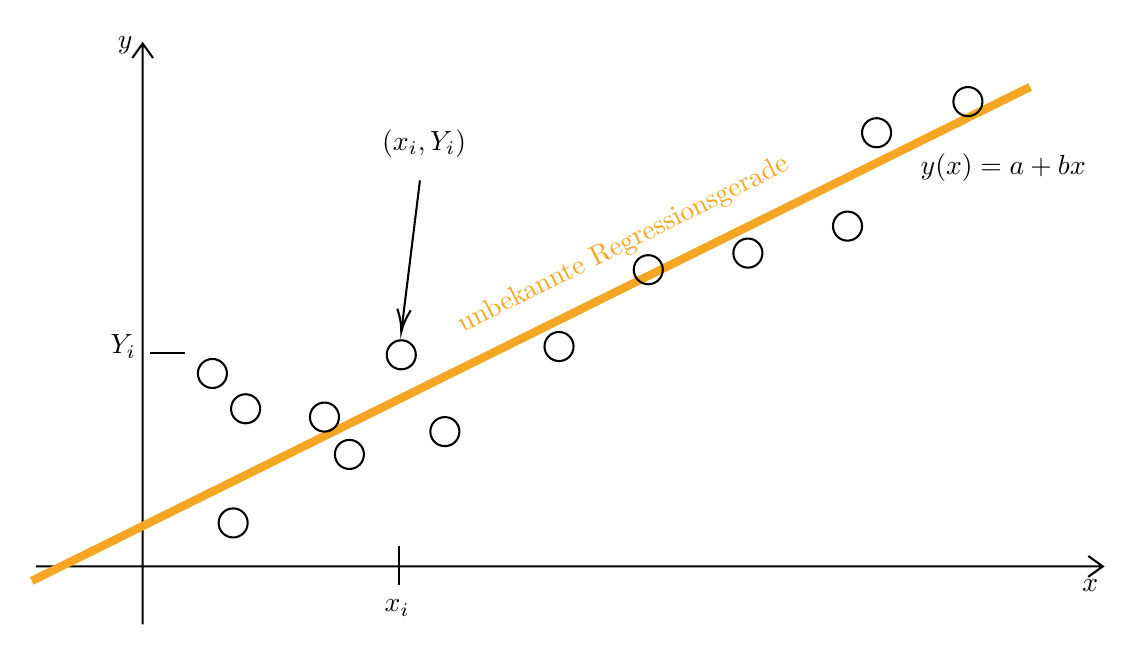
\begin{tikzpicture}[x=0.75pt,y=0.75pt,yscale=-1,xscale=1]
%uncomment if require: \path (0,300); %set diagram left start at 0, and has height of 300

%Shape: Axis 2D [id:dp07321911068108622] 
\draw  (4,261.94) -- (518,261.94)(55.4,10) -- (55.4,289.93) (511,256.94) -- (518,261.94) -- (511,266.94) (50.4,17) -- (55.4,10) -- (60.4,17)  ;
%Straight Lines [id:da07148662198339073] 
\draw [color={rgb, 255:red, 245; green, 166; blue, 35 }  ,draw opacity=1 ][line width=3]    (2,268.93) -- (483,30.93) ;


%Shape: Circle [id:dp26668633556271415] 
\draw   (92,241) .. controls (92,237.13) and (95.13,234) .. (99,234) .. controls (102.87,234) and (106,237.13) .. (106,241) .. controls (106,244.87) and (102.87,248) .. (99,248) .. controls (95.13,248) and (92,244.87) .. (92,241) -- cycle ;
%Shape: Circle [id:dp3403607469057863] 
\draw   (98,186) .. controls (98,182.13) and (101.13,179) .. (105,179) .. controls (108.87,179) and (112,182.13) .. (112,186) .. controls (112,189.87) and (108.87,193) .. (105,193) .. controls (101.13,193) and (98,189.87) .. (98,186) -- cycle ;
%Shape: Circle [id:dp4758519789604272] 
\draw   (194,197) .. controls (194,193.13) and (197.13,190) .. (201,190) .. controls (204.87,190) and (208,193.13) .. (208,197) .. controls (208,200.87) and (204.87,204) .. (201,204) .. controls (197.13,204) and (194,200.87) .. (194,197) -- cycle ;
%Shape: Circle [id:dp35126366068887793] 
\draw   (446,38) .. controls (446,34.13) and (449.13,31) .. (453,31) .. controls (456.87,31) and (460,34.13) .. (460,38) .. controls (460,41.87) and (456.87,45) .. (453,45) .. controls (449.13,45) and (446,41.87) .. (446,38) -- cycle ;
%Shape: Circle [id:dp6450412209324151] 
\draw   (402,53) .. controls (402,49.13) and (405.13,46) .. (409,46) .. controls (412.87,46) and (416,49.13) .. (416,53) .. controls (416,56.87) and (412.87,60) .. (409,60) .. controls (405.13,60) and (402,56.87) .. (402,53) -- cycle ;
%Shape: Circle [id:dp4264033728988835] 
\draw   (388,98) .. controls (388,94.13) and (391.13,91) .. (395,91) .. controls (398.87,91) and (402,94.13) .. (402,98) .. controls (402,101.87) and (398.87,105) .. (395,105) .. controls (391.13,105) and (388,101.87) .. (388,98) -- cycle ;
%Shape: Circle [id:dp41793329654483513] 
\draw   (292,119) .. controls (292,115.13) and (295.13,112) .. (299,112) .. controls (302.87,112) and (306,115.13) .. (306,119) .. controls (306,122.87) and (302.87,126) .. (299,126) .. controls (295.13,126) and (292,122.87) .. (292,119) -- cycle ;
%Shape: Circle [id:dp4914935297369122] 
\draw   (136,190) .. controls (136,186.13) and (139.13,183) .. (143,183) .. controls (146.87,183) and (150,186.13) .. (150,190) .. controls (150,193.87) and (146.87,197) .. (143,197) .. controls (139.13,197) and (136,193.87) .. (136,190) -- cycle ;
%Shape: Circle [id:dp23764538796154067] 
\draw   (173,160) .. controls (173,156.13) and (176.13,153) .. (180,153) .. controls (183.87,153) and (187,156.13) .. (187,160) .. controls (187,163.87) and (183.87,167) .. (180,167) .. controls (176.13,167) and (173,163.87) .. (173,160) -- cycle ;
%Shape: Circle [id:dp6151497769773182] 
\draw   (249,156) .. controls (249,152.13) and (252.13,149) .. (256,149) .. controls (259.87,149) and (263,152.13) .. (263,156) .. controls (263,159.87) and (259.87,163) .. (256,163) .. controls (252.13,163) and (249,159.87) .. (249,156) -- cycle ;
%Shape: Circle [id:dp6112008925466065] 
\draw   (148,208) .. controls (148,204.13) and (151.13,201) .. (155,201) .. controls (158.87,201) and (162,204.13) .. (162,208) .. controls (162,211.87) and (158.87,215) .. (155,215) .. controls (151.13,215) and (148,211.87) .. (148,208) -- cycle ;
%Shape: Circle [id:dp7443465654150703] 
\draw   (340,111) .. controls (340,107.13) and (343.13,104) .. (347,104) .. controls (350.87,104) and (354,107.13) .. (354,111) .. controls (354,114.87) and (350.87,118) .. (347,118) .. controls (343.13,118) and (340,114.87) .. (340,111) -- cycle ;
%Straight Lines [id:da5984247302071123] 
\draw    (179,251.93) -- (179,270.93) ;


%Straight Lines [id:da6676175412533971] 
\draw    (59,158.93) -- (76,158.93) ;


%Straight Lines [id:da2593592347170056] 
\draw    (189,75.93) -- (180.24,147.02) ;
\draw [shift={(180,149)}, rotate = 277.02] [color={rgb, 255:red, 0; green, 0; blue, 0 }  ][line width=0.75]    (10.93,-3.29) .. controls (6.95,-1.4) and (3.31,-0.3) .. (0,0) .. controls (3.31,0.3) and (6.95,1.4) .. (10.93,3.29)   ;

%Shape: Circle [id:dp9148664206548816] 
\draw   (82,169) .. controls (82,165.13) and (85.13,162) .. (89,162) .. controls (92.87,162) and (96,165.13) .. (96,169) .. controls (96,172.87) and (92.87,176) .. (89,176) .. controls (85.13,176) and (82,172.87) .. (82,169) -- cycle ;

% Text Node
\draw (470,70) node   {$y( x) =a+bx$};
% Text Node
\draw (287,107) node [rotate=-333.51] [align=left] {\textcolor[rgb]{0.96,0.65,0.14}{unbekannte Regressionsgerade}};
% Text Node
\draw (512,271) node   {$x$};
% Text Node
\draw (47,11) node   {$y$};
% Text Node
\draw (178,282) node   {$x_{i}$};
% Text Node
\draw (46,156) node   {$Y_{i}$};
% Text Node
\draw (191,58) node   {$( x_{i} ,Y_{i})$};


\end{tikzpicture}


			\caption{Einfache lineare Regression}
			%\label{Abb:MinQuaSchätzer}
		\end{center}
	\end{figure}
	
	\begin{figure}[H]
		\begin{center}
			% This work is licensed under the Creative Commons
% Attribution-NonCommercial-ShareAlike 4.0 International License. To view a copy
% of this license, visit http://creativecommons.org/licenses/by-nc-sa/4.0/ or
% send a letter to Creative Commons, PO Box 1866, Mountain View, CA 94042, USA.




% Pattern Info
 
\tikzset{
pattern size/.store in=\mcSize, 
pattern size = 5pt,
pattern thickness/.store in=\mcThickness, 
pattern thickness = 0.3pt,
pattern radius/.store in=\mcRadius, 
pattern radius = 1pt}
\makeatletter
\pgfutil@ifundefined{pgf@pattern@name@_yznbr6opy}{
\pgfdeclarepatternformonly[\mcThickness,\mcSize]{_yznbr6opy}
{\pgfqpoint{0pt}{0pt}}
{\pgfpoint{\mcSize+\mcThickness}{\mcSize+\mcThickness}}
{\pgfpoint{\mcSize}{\mcSize}}
{
\pgfsetcolor{\tikz@pattern@color}
\pgfsetlinewidth{\mcThickness}
\pgfpathmoveto{\pgfqpoint{0pt}{0pt}}
\pgfpathlineto{\pgfpoint{\mcSize+\mcThickness}{\mcSize+\mcThickness}}
\pgfusepath{stroke}
}}
\makeatother
\tikzset{every picture/.style={line width=0.75pt}} %set default line width to 0.75pt        

\begin{tikzpicture}[x=0.75pt,y=0.75pt,yscale=-1,xscale=1]
%uncomment if require: \path (0,300); %set diagram left start at 0, and has height of 300

%Shape: Axis 2D [id:dp17046936193864992] 
\draw  (50,264.53) -- (573,264.53)(102.3,8.93) -- (102.3,292.93) (566,259.53) -- (573,264.53) -- (566,269.53) (97.3,15.93) -- (102.3,8.93) -- (107.3,15.93)  ;
%Straight Lines [id:da10502832048562816] 
\draw [color={rgb, 255:red, 11; green, 17; blue, 252 }  ,draw opacity=1 ][line width=3]    (40,195.93) -- (529,43.93) ;


%Shape: Circle [id:dp3936057208076633] 
\draw  [fill={rgb, 255:red, 0; green, 0; blue, 0 }  ,fill opacity=1 ] (124,160.5) .. controls (124,158.01) and (126.01,156) .. (128.5,156) .. controls (130.99,156) and (133,158.01) .. (133,160.5) .. controls (133,162.99) and (130.99,165) .. (128.5,165) .. controls (126.01,165) and (124,162.99) .. (124,160.5) -- cycle ;
%Shape: Circle [id:dp7335662721698364] 
\draw  [fill={rgb, 255:red, 0; green, 0; blue, 0 }  ,fill opacity=1 ] (166,141.5) .. controls (166,139.01) and (168.01,137) .. (170.5,137) .. controls (172.99,137) and (175,139.01) .. (175,141.5) .. controls (175,143.99) and (172.99,146) .. (170.5,146) .. controls (168.01,146) and (166,143.99) .. (166,141.5) -- cycle ;
%Shape: Circle [id:dp10562516602478167] 
\draw  [fill={rgb, 255:red, 0; green, 0; blue, 0 }  ,fill opacity=1 ] (269,91.5) .. controls (269,89.01) and (271.01,87) .. (273.5,87) .. controls (275.99,87) and (278,89.01) .. (278,91.5) .. controls (278,93.99) and (275.99,96) .. (273.5,96) .. controls (271.01,96) and (269,93.99) .. (269,91.5) -- cycle ;
%Shape: Circle [id:dp6248807101111838] 
\draw  [fill={rgb, 255:red, 0; green, 0; blue, 0 }  ,fill opacity=1 ] (323,45.5) .. controls (323,43.01) and (325.01,41) .. (327.5,41) .. controls (329.99,41) and (332,43.01) .. (332,45.5) .. controls (332,47.99) and (329.99,50) .. (327.5,50) .. controls (325.01,50) and (323,47.99) .. (323,45.5) -- cycle ;
%Shape: Circle [id:dp719119066288937] 
\draw  [fill={rgb, 255:red, 0; green, 0; blue, 0 }  ,fill opacity=1 ] (144,180.5) .. controls (144,178.01) and (146.01,176) .. (148.5,176) .. controls (150.99,176) and (153,178.01) .. (153,180.5) .. controls (153,182.99) and (150.99,185) .. (148.5,185) .. controls (146.01,185) and (144,182.99) .. (144,180.5) -- cycle ;
%Shape: Circle [id:dp7264172592917753] 
\draw  [fill={rgb, 255:red, 0; green, 0; blue, 0 }  ,fill opacity=1 ] (364,28.5) .. controls (364,26.01) and (366.01,24) .. (368.5,24) .. controls (370.99,24) and (373,26.01) .. (373,28.5) .. controls (373,30.99) and (370.99,33) .. (368.5,33) .. controls (366.01,33) and (364,30.99) .. (364,28.5) -- cycle ;
%Shape: Circle [id:dp33818115228089896] 
\draw  [fill={rgb, 255:red, 0; green, 0; blue, 0 }  ,fill opacity=1 ] (51,210.5) .. controls (51,208.01) and (53.01,206) .. (55.5,206) .. controls (57.99,206) and (60,208.01) .. (60,210.5) .. controls (60,212.99) and (57.99,215) .. (55.5,215) .. controls (53.01,215) and (51,212.99) .. (51,210.5) -- cycle ;
%Shape: Circle [id:dp34245504510141156] 
\draw  [fill={rgb, 255:red, 0; green, 0; blue, 0 }  ,fill opacity=1 ] (283,64.5) .. controls (283,62.01) and (285.01,60) .. (287.5,60) .. controls (289.99,60) and (292,62.01) .. (292,64.5) .. controls (292,66.99) and (289.99,69) .. (287.5,69) .. controls (285.01,69) and (283,66.99) .. (283,64.5) -- cycle ;
%Shape: Circle [id:dp5914292952911566] 
\draw  [fill={rgb, 255:red, 0; green, 0; blue, 0 }  ,fill opacity=1 ] (223,114.5) .. controls (223,112.01) and (225.01,110) .. (227.5,110) .. controls (229.99,110) and (232,112.01) .. (232,114.5) .. controls (232,116.99) and (229.99,119) .. (227.5,119) .. controls (225.01,119) and (223,116.99) .. (223,114.5) -- cycle ;
%Shape: Circle [id:dp40497536712327753] 
\draw  [fill={rgb, 255:red, 0; green, 0; blue, 0 }  ,fill opacity=1 ] (82,214.5) .. controls (82,212.01) and (84.01,210) .. (86.5,210) .. controls (88.99,210) and (91,212.01) .. (91,214.5) .. controls (91,216.99) and (88.99,219) .. (86.5,219) .. controls (84.01,219) and (82,216.99) .. (82,214.5) -- cycle ;
%Shape: Circle [id:dp39909888798506066] 
\draw  [fill={rgb, 255:red, 0; green, 0; blue, 0 }  ,fill opacity=1 ] (237,149.5) .. controls (237,147.01) and (239.01,145) .. (241.5,145) .. controls (243.99,145) and (246,147.01) .. (246,149.5) .. controls (246,151.99) and (243.99,154) .. (241.5,154) .. controls (239.01,154) and (237,151.99) .. (237,149.5) -- cycle ;
%Shape: Circle [id:dp2019267403650239] 
\draw  [fill={rgb, 255:red, 0; green, 0; blue, 0 }  ,fill opacity=1 ] (348,74.5) .. controls (348,72.01) and (350.01,70) .. (352.5,70) .. controls (354.99,70) and (357,72.01) .. (357,74.5) .. controls (357,76.99) and (354.99,79) .. (352.5,79) .. controls (350.01,79) and (348,76.99) .. (348,74.5) -- cycle ;
%Shape: Circle [id:dp5259745267856665] 
\draw  [fill={rgb, 255:red, 0; green, 0; blue, 0 }  ,fill opacity=1 ] (294,113.5) .. controls (294,111.01) and (296.01,109) .. (298.5,109) .. controls (300.99,109) and (303,111.01) .. (303,113.5) .. controls (303,115.99) and (300.99,118) .. (298.5,118) .. controls (296.01,118) and (294,115.99) .. (294,113.5) -- cycle ;
%Shape: Circle [id:dp17390342487641564] 
\draw  [fill={rgb, 255:red, 0; green, 0; blue, 0 }  ,fill opacity=1 ] (416,112.5) .. controls (416,110.01) and (418.01,108) .. (420.5,108) .. controls (422.99,108) and (425,110.01) .. (425,112.5) .. controls (425,114.99) and (422.99,117) .. (420.5,117) .. controls (418.01,117) and (416,114.99) .. (416,112.5) -- cycle ;
%Shape: Circle [id:dp23479676072523903] 
\draw  [fill={rgb, 255:red, 0; green, 0; blue, 0 }  ,fill opacity=1 ] (401,29.5) .. controls (401,27.01) and (403.01,25) .. (405.5,25) .. controls (407.99,25) and (410,27.01) .. (410,29.5) .. controls (410,31.99) and (407.99,34) .. (405.5,34) .. controls (403.01,34) and (401,31.99) .. (401,29.5) -- cycle ;
%Straight Lines [id:da34048831480133634] 
\draw [color={rgb, 255:red, 245; green, 166; blue, 35 }  ,draw opacity=1 ][line width=1.5]    (368.5,28.5) -- (391,86.93) ;


%Straight Lines [id:da8628989912348813] 
\draw [color={rgb, 255:red, 245; green, 166; blue, 35 }  ,draw opacity=1 ][line width=1.5]    (352.5,74.5) -- (358,92.93) ;


%Straight Lines [id:da6248165946669281] 
\draw [color={rgb, 255:red, 245; green, 166; blue, 35 }  ,draw opacity=1 ][line width=1.5]    (327.5,45.5) -- (345,97.93) ;


%Straight Lines [id:da057361574656471515] 
\draw [color={rgb, 255:red, 245; green, 166; blue, 35 }  ,draw opacity=1 ][line width=1.5]    (287.5,64.5) -- (303,113.5) ;


%Straight Lines [id:da9723378016055195] 
\draw [color={rgb, 255:red, 245; green, 166; blue, 35 }  ,draw opacity=1 ][line width=1.5]    (273.5,91.5) -- (283,119.93) ;


%Straight Lines [id:da7072892699379895] 
\draw [color={rgb, 255:red, 245; green, 166; blue, 35 }  ,draw opacity=1 ][line width=1.5]    (227.5,114.5) -- (241.5,149.5) ;


%Straight Lines [id:da5331650878440136] 
\draw [color={rgb, 255:red, 245; green, 166; blue, 35 }  ,draw opacity=1 ][line width=1.5]    (170.5,141.5) -- (176,150.93) ;


%Straight Lines [id:da2225989489764092] 
\draw [color={rgb, 255:red, 245; green, 166; blue, 35 }  ,draw opacity=1 ][line width=1.5]    (148.5,180.5) -- (144,163.93) ;


%Straight Lines [id:da30768836888532625] 
\draw [color={rgb, 255:red, 245; green, 166; blue, 35 }  ,draw opacity=1 ][line width=1.5]    (128.5,160.5) -- (128.5,165) ;


%Straight Lines [id:da9543043664995713] 
\draw [color={rgb, 255:red, 245; green, 166; blue, 35 }  ,draw opacity=1 ][line width=1.5]    (86.5,214.5) -- (76,184.93) ;


%Straight Lines [id:da3131414955517793] 
\draw [color={rgb, 255:red, 245; green, 166; blue, 35 }  ,draw opacity=1 ][line width=1.5]    (55.5,210.5) -- (48,193.93) ;


%Shape: Square [id:dp4250994342007913] 
\draw  [color={rgb, 255:red, 245; green, 166; blue, 35 }  ,draw opacity=1 ][pattern=_yznbr6opy,pattern size=6pt,pattern thickness=0.75pt,pattern radius=0pt, pattern color={rgb, 255:red, 245; green, 166; blue, 35}][line width=1.5]  (405.5,29.5) -- (452.86,13.48) -- (468.89,60.84) -- (421.52,76.86) -- cycle ;
%Straight Lines [id:da5455233967320696] 
\draw    (409,255.93) -- (409,274.93) ;


%Straight Lines [id:da8891249987228257] 
\draw [color={rgb, 255:red, 245; green, 166; blue, 35 }  ,draw opacity=1 ][line width=1.5]    (410,82.93) -- (420.5,112.5) ;


%Straight Lines [id:da2990647448398298] 
\draw    (93,34.93) -- (110,34.93) ;



% Text Node
\draw (410,281) node   {$x_{i}$};
% Text Node
\draw (515,22) node   {$Y_{i} -( \alpha +\beta \cdot x_{i})$};
% Text Node
\draw (68,23) node   {$\alpha +\beta \cdot x_{i}$};


\end{tikzpicture}

			\caption{Einfache lineare Regression - Methode der kleinsten Fehlerquadrate}
			%\label{Abb:MinQuaSchätzer}
		\end{center}
	\end{figure}

	\begin{align*}
		\underbrace{\begin{pmatrix}
			Y_1\\
			\vdots\\
			\vdots\\
			Y_n
		\end{pmatrix}}_{=Y}
		&=\underbrace{\begin{pmatrix}
			1 & x_1\\
			\vdots & x_2\\
			\vdots & \vdots\\
			1 & x_n
		\end{pmatrix}}_{=X}\mal\underbrace{\begin{pmatrix}
			a\\
			b
		\end{pmatrix}}_{=\beta}+\underbrace{\begin{pmatrix}
			\varepsilon_1\\
			\vdots\\
			\vdots\\
			\varepsilon_n
		\end{pmatrix}}_{=\varepsilon}
	\end{align*}
	Angenommen, $\Rg(X)=2$ ($\overset{!}{\iff}\exists i\neq j:x_i\neq x_j$)
	\begin{align*}
		X'\mal X
		&=\begin{pmatrix}
			1 & \hdots & 1\\
			x_1 & \hdots & x_n
		\end{pmatrix}\mal\begin{pmatrix}
			1 & x_1\\
			\vdots &  \vdots\\
			1 & x_n
		\end{pmatrix}
		=\begin{pmatrix}
			n & \sum\limits_{i=1}^n x_i\\
			\sum\limits_{i=1}^n x_i & \sum\limits_{i=1}^n x_i^2
		\end{pmatrix}
		=\begin{pmatrix}
			n & n\mal\overline{x_n}\\
			n\mal\overline{x_n} & \sum\limits_{i=1}^n x_i^2
		\end{pmatrix}\\
		X'\mal Y
		&=\begin{pmatrix}
			1 & \hdots & 1\\
			x_1 & \hdots & x_n
		\end{pmatrix}\mal\begin{pmatrix}
			Y_1\\
			\vdots\\
			Y_n
		\end{pmatrix}
		=\begin{pmatrix}
			\sum\limits_{i=1}^n Y_i\\
			\sum\limits_{i=1}^n x_i\mal Y_i
		\end{pmatrix}
		=\begin{pmatrix}
			n\mal\overline{Y_n}\\
			\sum\limits_{i=1}^n x_i\mal Y_i
		\end{pmatrix}\\
		\mit\qquad \overline{x_n}&:=\frac{1}{n}\mal\sum\limits_{i=1}^n x_i
		\qquad\und\qquad
		\overline{Y_n}:=\frac{1}{n}\mal\sum\limits_{i=1}^n Y_i
	\end{align*}
	Normalgleichung \eqref{eq:satz3.3Stern}:
	\begin{align*}
		\begin{pmatrix}
			n & n\mal\overline{x_n}\\
			n\mal\overline{x_n} & \sum\limits_{i=1}^n x_i^2
		\end{pmatrix}\mal\begin{pmatrix}
			\alpha\\
			\beta
		\end{pmatrix}=\begin{pmatrix}
			n\mal\overline{Y_n}\\
			\sum\limits_{i=1}^n x_i\mal Y_i
		\end{pmatrix}\\
		\iff
		\left\lbrace\begin{array}{l}
			(1)~~
			n\mal\alpha+n\mal\overline{x_n}\mal\beta=n\mal\overline{Y_n}
			\iff\alpha=\overline{Y_n}-\overline{x_n}\mal\beta\\
			(2)~~n\mal\overline{x_n}\mal\alpha+\sum\limits_{i=1}^n x_i^2\mal\beta=\sum\limits_{i=1}^n x_i\mal Y_i
		\end{array}\right.
	\end{align*}
	Teilen durch $n$ in (2) und einsetzen von (1) in (2) liefert:
	\begin{align*}
		\overline{x_n}\mal \overline{Y_n}\underbrace{-\overline{x_n}^2\mal\beta+\frac{1}{n}\mal\sum\limits_{i=1}^n x_i^2\mal\beta}_{
			=\beta\mal\klammern{\frac{1}{n}\mal\sum\limits_{i=1}^n \big(x_i^2-\overline{x_n}^2\big)}
		}
		&=\frac{1}{n}\mal\sum\limits_{i=1}^n x_i\mal Y_i\\
		\implies
		\beta
		&=\frac{
			\frac{1}{n}\mal\sum\limits_{i=1}^n x_i\mal Y_i-\overline{x_n}\mal\overline{Y_n}
		}{
			\frac{1}{n}\mal\sum\limits_{i=1}^n \big(x_i^2-\overline{x_n}^2\big)
		}\\
		&=
		\frac{
			\frac{1}{n}\mal\klammern{\sum\limits_{i=1}^n x_i\mal Y_i-n\mal\overline{x_n}\mal\overline{Y_n}}
		}{
			\frac{1}{n}\mal\sum\limits_{i=1}^n \big(x_i^2-\overline{x_n}^2\big)
		}\\
		\overset{\mal\frac{n}{n-1}}&{=}
		\frac{
			\frac{1}{n-1}\mal\klammern{\sum\limits_{i=1}^n x_i\mal Y_i-n\mal\overline{x_n}\mal\overline{Y_n}}		
		}{
			\frac{1}{n-1}\mal\klammern{\sum\limits_{i=1}^n x_i^2-n\mal \overline{x_n}^2}
		}\\
		\overset{!}&{=}
		\frac{
			\frac{1}{n-1}\mal\sum\limits_{i=1}^n\big(x_i-\overline{x_n}\big)\mal\big(Y_i-\overline{Y_n}\big)
		}{
			\frac{1}{n-1}\mal \sum\limits_{i=1}^n\big(x_i-\overline{x_n}\big)^2
		}\\
		&=:\frac{s_{x,Y}}{s_x^2}
	\end{align*}
	Hierbei heißen $s_{x,Y}$ \define{empirische Kovarianz} und $s_x^2$ \define{empirische Varianz}.
	\index{empirische Varianz}\index{empirische Kovarianz}
	\begin{align*}
		\hat{\beta}=\begin{pmatrix}
			\hat{a}\\
			\hat{b}
		\end{pmatrix}\qquad\mit\qquad
		\hat{a}:=\overline{Y_n}-\overline{x_n}\mal\hat{b},\qquad
		\hat{b}:=\frac{s_{x,Y}}{s_x^2}
	\end{align*}
\end{beispiel}

\subsection{Optimalität des MQS} %3.2

Betrachten im linearen Modell $Y=X\mal\beta+\varepsilon$ \define{lineare} Funktionen $\Psi$ von $\beta$, d.h.
\begin{align*}
	\Psi\colon\R^p\to\R,\qquad\Psi(\beta)=c'\mal\beta\qquad\forall \beta	\in\R^p,
\end{align*}
wobei $c\in\R^p$ fest vorgegeben (bekannt).

\begin{beisp}\
	\begin{enumerate}[label=(\arabic*)]
		\item $\begin{aligned}
			c=e_j\implies\Psi(\beta)=e_j'\mal\beta=\beta_j
		\end{aligned}$
		\item $\begin{aligned}
			c=e_i-e_j\implies\Psi(\beta)=\beta_i-\beta_j
		\end{aligned}$
	\end{enumerate}
\end{beisp}

\begin{definition}\label{def3.6}\
	\begin{enumerate}[label=(\arabic*)]
		\item $\Psi(\beta)=c'\mal\beta$ heißt \define{schätzbar} $\defiff\exists a\in\R^n$ so, dass
		\index{schätzbar}
		\begin{align*}
			\hat{\Psi}:=a'\mal Y=\sum\limits_{i=1}^n a_i\mal Y_i
		\end{align*}
		ein \define{erwartungstreuer Schätzer} für $\Psi$ ist, d.h.
		\index{erwartungstreuer Schätzer}
		\begin{align*}
			\E_\beta\big[\hat{\Psi}\big]=\Psi(\beta)\qquad\forall \beta\in\R^p
		\end{align*}
		\item Schätzer der Form $a'\mal Y$ heißen \define{lineare Schätzer}.
		\index{lineare Schätzer}
	\end{enumerate}
	Kurz: $c'\mal\beta$ ist schätzbar $\iff\exists$ linearer und erwartungstreuer Schätzer für $c'\mal\beta$.
\end{definition}

\begin{lemma}\label{lemma3.7}\
	\begin{enumerate}[label=(\arabic*)]
		\item $\begin{aligned}
			\Psi(\beta)=c'\mal\beta
		\end{aligned}$ schätzbar $\iff\exists a\in\R^n$ mit
		\label{item:lemma3.7(1)}
		\begin{align}\label{eq:3.7}\tag{3.7}
			c'=a'\mal X\qquad\Big(\iff c=X'\mal a\Big)
		\end{align}
		d.h.
		\begin{align*}
			c\in\Bild(X')=\set{X'\mal y:y\in\R^n}
		\end{align*}
		\item Falls $\Rg(X)=p$ (also Vollrang), so ist $c'\mal\beta$ für alle $c\in\R^p$ schätzbar.
		\label{item:lemma3.7(2)}
	\end{enumerate}
\end{lemma}

\begin{proof}
	\betone{Zu \ref{item:lemma3.7(1)} zeige "$\Longrightarrow$":}\\
	Es existiert $a\in\R^n$ so, dass:
	\begin{align*}
		c'\mal\beta
		&=\E[a'\mal Y]
		\overset{\Lin}{=}
		a'\mal\E[Y]
		=a'\mal X\mal\beta &&\forall\beta\in\R^p\\
		\overset{\beta:=e_j}{\iff}
		c'&=a'\mal X
	\end{align*}		
	
	\betone{Zu \ref{item:lemma3.7(1)} zeige "$\Longleftarrow$":}\\
	Es ist $\hat{\Psi}:=a'\mal Y$ ein linearer Schätzer und es gilt:
	\begin{align*}
		\E\big[\hat{\Psi}\big]
		&=a'\mal\E[Y]
		=\underbrace{a'\mal X}_{
			\overset{\eqref{eq:3.7}}{=}c'		
		}\mal\beta
		=c'\mal\beta
		=\Psi(\beta)
		\qquad\forall \beta\in\R^p
	\end{align*}
	Also ist $c'\mal\beta$ schätzbar.\nl
	\betone{Zeige \ref{item:lemma3.7(2)}:}\\
	Setze
	\begin{align*}
		a':=c'\mal\big(X'\mal X\big)^{-1}\mal X'.
	\end{align*}
	Die Inverse hier existiert wegen Satz \ref{satz:2.13}.
	Dann gilt:
	\begin{align*}
		a'\mal X
		&=c'
		\overset{\ref{item:lemma3.7(1)}}{\implies}\text{ Behauptung}
	\end{align*}
\end{proof}

\begin{lemma}\label{lemma3.8}
	Sei $\Psi(\beta)=c'\mal\beta$ schätzbar.
	Dann gilt:
	\begin{enumerate}[label=(\arabic*)]
		\item Es existiert ein $b\in\R^n$ mit
		\begin{align}\label{eq:lemma3.8Stern}\tag{$*$}
			b'\mal Y\text{ ist erwartungstreu für }\Psi
		\end{align}
		\label{item:lemma3.8(1)}
		\item Es existiert genau ein $a\in L:=\Bild(X)\subseteq\R^n$ derart, dass
		\label{item:lemma3.8(2)}
		\begin{align*}
			\hat{\Psi}:=a'\mal Y
		\end{align*}
		erwartungstreu für $\Psi$ ist, nämlich
		\begin{align*}
			a=P_L(b)
		\end{align*}
		für jedes $b$ mit \eqref{eq:lemma3.8Stern}.
	\end{enumerate}
\end{lemma}

\begin{proof}
	\betone{Zeige \ref{item:lemma3.8(1)}:}\\
	Gilt gemäß Definition \ref{def3.6}.\nl
	\betone{Zeige \ref{item:lemma3.8(2)}:}
	\begin{align*}
		b&=a+\tilde{a},\qquad a=P_L(b)\in L,~\tilde{a}\in L^\perp
	\end{align*}
	Es gilt für alle $\beta\in\R^p$:
	\begin{align*}
		\Psi(\beta)
		\overset{\ref{item:lemma3.8(1)}}&{=}
		\E[b'\mal Y]\\
		&=b'\mal X\mal\beta\\
		&=\big(a'+\tilde{a}'\big)\mal X\mal\beta\\
		&=a'\mal X\mal\beta+\underbrace{\tilde{a}'\mal X\mal\beta}_{
			=\scaProd[\big]{\tilde{a}}{\underbrace{X\mal\beta}_{\in L}}
			\overset{\tilde{a}\in L^\perp}{=}0
		}\\
		&=a'\mal\underbrace{X\mal\beta}_{
			=\E[Y]
		}\\
		\overset{\Lin}&{=}
		\E[a'\mal Y]
	\end{align*}
	Somit folgt
	\begin{align}\label{eq:ProofLemma3.8Plus}\tag{+}
		\hat{\Psi}:=a'\mal Y\text{ ist erwartungatreu für $\Psi$ mit }a=P_L(b)\in L
	\end{align}
	Bleibt Eindeutigkeit zu zeigen:
	Sei $\overline{a}\in L$ mit $\overline{a}'\mal Y$ ist erwartungstreu für $\Psi$.
	Dann folgt:
	\begin{align*}
		&a'\mal X\mal\beta
		\overset{\Lin}{=}
		\E[a'\mal Y]
		\overset{\eqref{eq:ProofLemma3.8Plus}}{=}
		c'\mal\beta
		=\E[\overline{a}'\mal Y]
		\overset{\Lin}{=}
		\overline{a}'\mal X\mal\beta
		&&\forall \beta\in\R^p\\
		&\implies
		0=\big(a'-\overline{a}'\big)\mal X\mal\beta
		=\big(a-\overline{a}\big)'\mal X\mal\beta&&\forall\beta\in\R^p\\
		&\implies a-\overline{a}\in L^\perp
	\end{align*}
	Aber $a-\overline{a}\in L$, da $L$ Untervektorraum.
	Somit ist 
	\begin{align*}
		a-\overline{a}\in L^\perp\cap L\overset{\ref{satz2.1}\ref{item:satz2.1(3)}\ref{item:satz2.1(3i)}}{=}
	\set{0}
	\implies \overline{a}=a
	\end{align*}		
\end{proof}

\begin{satz}[Gauß-Markov-Theorem]\label{satz3.9GaussMarkovTheorem}\enter
	Sei $\Psi(\beta)=c'\mal\beta$ schätzbar und $\hat{\Psi}:=c'\mal\beta$, $\hat{\beta}=$ MQS für $\beta$.
	Dann gilt:
	\begin{enumerate}[label=(\arabic*)]
		\item $\hat{\Psi}$ ist linearer und erwarungstreuer Schätzer für $\Psi$ und der einzige unter allen linearen erwarungstreuen Schätzern für $\psi$ mit \betone{minimaler Varianz}.
		\label{item:satz3.9(1)}
		\item $\hat{\Psi}=a'\mal Y$ für ein eindeutig bestimmtes $a\in L$ und 
		\label{item:satz3.9(2)}
		\begin{align*}
			\Var\big(\hat{\Psi}\big)=\sigma^2\mal\norm{a}^2
		\end{align*}
	\end{enumerate}
\end{satz}

\begin{proof}
	Gemäß Lemma \ref{lemma3.8} existiert genau ein $a\in L$ mit
	%\begin{enumerate}[label=(\roman*)]
	\begin{align}\label{eq:ProofSatz3.9(i)}\tag{i}
		a'\mal Y\text{ erwartungstreu für }\Psi
	\end{align}
		%\item $a'\mal Y$ erwartungstreu für $\Psi$
	%\end{enumerate}
	Es gilt
	\begin{align}\label{eq:ProofSatz3.9RoterStern}\tag{$*$}
		a'\mal Y
		\overset{a\in L,\ref{satz2.5}\ref{item:satz2.5(2)}}&{=}
		\big(P_L a\big)'\mal Y
		=a'\mal P_L' Y
		\overset{\ref{satz2.8}\ref{item:satz2.8(2)}}{=}
		a'\mal\underbrace{P_L Y}_{
			=X\mal\hat{\beta}
		}
		\overset{\ref{satz3.3}\ref{item:satz3.3(1)}}{=}
		a'\mal X\mal\hat{\beta}
	\end{align}
	Ferner gilt:
	\begin{align*}
		a'\mal X\mal\beta
		&=a'\mal\E[Y]
		\overset{\Lin}{=}
		\E[a'\mal Y]
		\overset{\eqref{eq:ProofSatz3.9(i)}}{=}
		c'\mal\beta
		\qquad\forall\beta\in\R^p
	\end{align*}
	Wende nun \eqref{eq:ProofSatz3.9RoterStern} mit $\beta:=\hat{\beta}$ an:
	\begin{align}\label{eq:ProofSatz3.9(ii)}\tag{ii}
		a'\mal Y=c'\mal\beta=\hat{\Psi}
	\end{align}
	Also ist $\hat{\Psi}$ linearer erwartungstreuer Schätzer für $\Psi$.
	Ferner:
	\begin{align}\label{eq:ProofSatz3.9(iii)}\tag{iii}
		\Var(\hat{\Psi})
		&=\Var(a'\mal Y)
		\overset{\ref{satz3.2}\ref{item:satz3.2(2)}}{=}
		a'\mal\underbrace{\Var(Y)}_{
			\overset{\ref{satz3.2}}{=}
			\Var(\varepsilon)
			\overset{\eqref{eq:3.2}}{=}
			\sigma^2\mal I_n
		}\mal a
		=\sigma^2\mal\norm{a}^2
	\end{align}

	Sei $\tilde{\Psi}=b'\mal Y$ ein beliebiger linearer, erwartungstreuer Schätzer für $\Psi$.
	Dann folgt (vergleiche \eqref{eq:ProofSatz3.9(iii)}):
	\begin{align}\label{eq:ProofSatz3.9(iii)Strich}\tag{iii'}
		\Var(\tilde{\Psi})=\sigma^2\mal\norm{b}^2
	\end{align}
	Es gilt:
	\begin{align}\label{eq:ProofSatz3.9SternStern}\tag{$**$}
		b&=P_L(b)+v
		\overset{\ref{lemma3.8}\ref{item:lemma3.8(2)}}{=}
		a+v\qquad v\in L^\perp
	\end{align}
	Dann folgt aus Pythagoras:
	\begin{align}\label{eq:ProofSatz3.9(iv)}\tag{iv}
		\norm{b}^2
		\overset{\text{Pythago}}&{=}
		\norm{a}^2+\norm{v}^2
		\geq\norm{a}^2
		\overset{\eqref{eq:ProofSatz3.9(iii)},\eqref{eq:ProofSatz3.9(iii)Strich}}{\implies}
		\Var(\tilde{\Psi})=\Var(\hat{\Psi})
	\end{align}
	 \betone{Eindeutigkeit:}\\
	 Angenommen $\tilde{\Psi}=b'\mal Y$ hat Minimalvarianz.
	 Dann gilt:
	 \begin{align*}
	 	\norm{a}^2=\norm{b}^2
	 	\implies\norm{v}^2=0
	 	\implies v=0
	 	\overset{\eqref{eq:ProofSatz3.9SternStern}}{\implies}
	 	b=a
	 	\overset{\eqref{eq:ProofSatz3.9(i)}}{=} %könnte auch (ii) sein
		\tilde{\Psi}=\hat{\Psi}
	 \end{align*}
	Gemeinsam mit \eqref{eq:ProofSatz3.9(i)}, \eqref{eq:ProofSatz3.9(ii)}, \eqref{eq:ProofSatz3.9(iii)} und \eqref{eq:ProofSatz3.9(iv)} folgen die Behauptungen.

	%\betone{Zeige \ref{item:satz3.9(1)}:}\\
	
	%\betone{Zeige \ref{item:satz3.9(2)}:}\\
\end{proof}

\begin{bemerkungnr}\label{bemerkung3.10}\
	\begin{enumerate}[label=(\arabic*)]
		\item In Satz \ref{satz3.9GaussMarkovTheorem} wird \betone{nicht} $\Rg(X)=p$ (also Vollrang) gefordert.
		\label{item:bem3.10_1}
		\item Sprechweise im Englischen: $c'\mal\hat{\beta}$ is \define{BLUE}
		 (:= best linear unbiased estimator)\\
		 "unbiased" wird mit "unverzerrt" übersetzt, was einfach erwartungstreu bedeutet.
		 \label{item:bem3.10_2}
		 \item Falls $\Rg(X)=p$ (also Vollrang), dann gilt:
		 \begin{align*}
		 	\Var(\hat{\Psi})=\Var\big(c'\mal\hat{\beta}\big)
		 	\overset{\ref{satz3.2}}{=}
		 	c'\mal\underbrace{\Var(\hat{\beta})}_{
		 		\overset{\ref{def3.6}}{=}\sigma^2\mal\big(X'\mal X\big)^{-1}
		 	}=\sigma^2\mal c'\mal(X'\mal X)^{-1}\mal c
		 \end{align*}
		 \label{item:bem3.10_3}
		 \item Speziell für $c=e_j$ liefert $\hat{\beta}_j=j$-te Komponente von $\hat{\beta}$ ist der BLUE für $\beta_j$
		 \label{item:bem3.10_4}
	\end{enumerate}
\end{bemerkungnr}

\subsection{Schätzung von \texorpdfstring{$\sigma^2$}{Sigma Quadrat}}
Wegen \eqref{eq:3.2} und \eqref{eq:3.3} gilt
\begin{align*}
	\sigma^2=\Var(\varepsilon_i)=\E[\varepsilon^2]\qquad\forall i\in\set{1,\ldots,n}
\end{align*}
Es folgt:
\begin{align*}
	\E\eckigeKlammern{\frac{1}{n}\mal\sum\limits_{i=1}^n\varepsilon_i^2}
	\overset{\Lin}{=}\E[\varepsilon_i^2]=\sigma^2
\end{align*}
Aber 
$
	\frac{1}{n}\mal\sum\limits_{i=1}^n\varepsilon_i^2
$
ist \betone{kein Schätzer} für $\sigma^2$, da der Fehlervektor 
$
	\varepsilon=\klammern[\big]{\varepsilon_1,\ldots,\varepsilon_n}
$\\1
\betone{nicht beobachtbar}.
\betone{Idee}:
Ersetze
$
	\varepsilon
	\overset{\eqref{eq:3.1}}{=}
	Y-X\mal\beta
$
durch \betone{bekanntes}
\begin{align*}
	\hat{\varepsilon}:=Y-X\mal\hat{\beta}=Y-\hat{Y},
\end{align*}
wobei 
$	
	\hat{Y}:=X\mal\hat{\beta}
$
das \define{den Daten angepassten (fitted)} $Y$.
$\hat{\varepsilon}$ heißt Vektor der \define{Residuen} (geschätzte Fehler).
\index{Residuenvektor}\\
Erhalte (bis auf Faktor $\frac{1}{n}$):
\begin{align*}
	\RSS:=\sum\limits_{i=1}^n\hat{\varepsilon}_i^2
	=\hat{\varepsilon}'\mal\hat{\varepsilon}
	=\norm{\hat{\varepsilon}}^2
\end{align*}
Das RSS steht für \define{Residual sums of squares} also \define{Residuenquadratsumme}.
\index{Residuenquadratsumme}

\begin{satz}\label{satz3.11}
	Sei $\Rg(X)=p<n$. Dann gilt:
	\begin{align*}
		\S^2:=\frac{1}{n-p}\mal\RSS>0
	\end{align*}
	ist \betone{erwartungstreuer} Schätzer für $\sigma^2$, d.h.
	\begin{align*}
		\E_\beta[S^2]=\sigma^2\qquad\forall \beta\in\R^p
	\end{align*}
\end{satz}

Zwei Hilfsmittel für den Beweis von Satz \ref{satz3.11}:

\begin{lemma}\label{lemma3.12}
	Sei $\Rg(X)=p$. 
	Dann gilt mit $L:=\Bild(X)$:
	\begin{align*}
		\Rg\big(I_n-P_L\big)
		=\Spur\big(I_n-P_L\big)
		=n-p
	\end{align*}
\end{lemma}

\begin{proof}
	\begin{align*}
		I_n-P_L
		\overset{\ref{satz2.9}}&{=}
		P_{L^\perp}
	\end{align*}
	Also ist $I_n-P_L$ symmetrische und idempotente Matrix gemäß Satz \ref{satz2.7} und Satz \ref{satz2.8}.
	Also ist
	\begin{align*}
		\Rg\big(I_n-P_L\big)
		\overset{\ref{satz2.1}\ref{item:satz2.1(2)}}&{=}
		\Spur\big(I_n-P_L\big)\\
		\overset{\Spur\text{ additiv}}&{=}
		\Spur(I_h)-\Spur(P_L)\\
		&=n-\Spur(P_L)\\
		\overset{\ref{satz3.3}\ref{item:satz3.3(2)}}&{=}
		n-\Spur\Big(X\mal\big(X'\mal X\big)^{-1}\mal X'\Big)\\
		\overset{\ref{satz2.14}}&{=}
		n-\Spur(I_p)\\
		&=n-p
	\end{align*}
\end{proof}

\begin{lemma}\label{lemma3.13}
	Sei $A\in M(n\times n)$ deterministisch und $Z$ ein Zufallsvektor in $\R^n$.
	Dann gilt für den Erwartungswert der quadratischen Form:
	\begin{align*}
		\E\eckigeKlammern[\big]{Z'\mal A\mal Z}
		=\Spur\klammern[\big]{A\mal\Var(Z)}+
		\E[Z]'\mal A\mal\E[Z]
	\end{align*}
\end{lemma}

\begin{proof}
	Setze $\theta:=\E[Z]$.
	Idee: Wir betrachten den zentrierten Vektor.
	\begin{align}\nonumber
		\E\eckigeKlammern[\big]{(Z-\theta)'\mal A\mal\underbrace{(Z-\theta)}_{
			\text{zentriert}
		}}
		&=\E\eckigeKlammern{Z'\mal A\mal Z-\theta'\mal A\mal Z-Z'\mal A\mal\theta+\theta'\mal A\mal\theta}\\\nonumber
		\overset{\ref{satz3.2}}&{=}
		\E\eckigeKlammern{Z'\mal A\mal Z}-\theta'\mal A\mal\underbrace{\E[Z]}_{=\theta}-\E[Z]'\mal A\mal\theta+\theta'\mal A\mal\theta\\\nonumber
		&=\E\eckigeKlammern{Z'\mal A\mal Z}-\theta'\mal A\mal\theta\\
		\implies
		\E\eckigeKlammern{Z'\mal A\mal Z}
		&=\underbrace{\E\eckigeKlammern[\big]{(Z-\theta)'\mal A\mal(Z-\theta)}}_{=:\mu}+\theta'\mal A\mal\theta
		\label{eqProofLemma3.13Stern}\tag{$*$}
	\end{align}
	Jetzt rechnen wir $\mu$ aus:
	\begin{align*}
		\mu&=\E\eckigeKlammern{\sum\limits_{1\leq i,j\leq n}\big(Z_i-\theta_i\big)\mal A_{i,j}\mal\big(Z_j-\theta_j\big)}\\
		\overset{\Lin}&{=}
		\sum\limits_{1\leq i,j\leq n}A_{i,j}\mal\E\eckigeKlammern[\Big]{\big(Z_i-\underbrace{\theta_i}_{=\E[Z_i]}\big)\mal\big(Z_j-\underbrace{\theta_j}_{=\E[Z_j]}\big)}\\
		&=\sum\limits_{1\leq i,j\leq n}A_{i,j}\mal\Cov\big(Z_i,Z_j\big)\\
		&=\sum\limits_{1\leq i,j\leq n}A_{i,j}\mal\big(\Var(Z)\big)_{i,j}\\
		\overset{\text{Symm}}&{=}
		\sum\limits_{i=1}^n\sum\limits_{j=1}^n A_{i,j}\mal\big(\Var(Z)\big)_{j,i}\\
		&=\sum\limits_{i=1}^n\klammern{\sum\limits_{j=1}^n A_{i,j}\mal\big(\Var(Z)\big)_{j,i}}\\
		&=\sum\limits_{i=1}^n\Big(A\mal \Var(Z)\Big)_{i,i}\\
		&=\Spur\big(A\mal\Var(Z)\big)
	\end{align*}
	Aus \eqref{eqProofLemma3.13Stern} folgt die Behauptung.
\end{proof}

\begin{proof}[Beweis von Satz \ref{satz3.11}]%\enter
	\begin{align*}
		\hat{\varepsilon}
		\overset{\Def}&{=}
		Y-X\mal\hat{\beta}
		\overset{\ref{satz3.3}}{=}
		Y-P_L Y
		=\big(I_n-P_L\big)Y
		\overset{\ref{satz2.9}}{=}
		P_{L^\perp}Y\\
		\implies
		(n-p)\mal S^2
		\overset{\Def}&{=}
		\RSS\\
		&=\hat{\varepsilon}'\mal\hat{\varepsilon}\\
		&=\big(P_{L^\perp} Y\big)'\mal\big(P_{L^\perp} Y\big)\\
		&=Y'\mal P_{L^\perp}'\mal P_{L^\perp}\mal Y\\
		\overset{\text{Symm}}&{=}
		Y'\mal P_{L^\perp}\mal P_{L^\perp}\mal Y\\
		\overset{\text{Idempotenz}}&{=}
		Y'\mal P_{L^\perp}\mal Y\\
		\implies
		(n-p)\mal\E\big[S^2\big]
		&=\E\eckigeKlammern{Y'\mal\big(I_n-P_L)\mal Y}\\
		\overset{\ref{lemma3.13}}&{=}
		\Spur\klammern[\Big]{\big(I_n-P_L\big)\mal\underbrace{\Var(Y)}_{
			=\sigma^2\mal I_n		
		}}+\underbrace{\E[Y]'\mal\underbrace{\big(I_h-P_L\big)}_{
			=P_{L^\perp}
		}\underbrace{\mal\E[Y]}_{
			=X\mal\beta\in L
		}}_{
			=0
		}\\
		&=\sigma^2\mal\Spur(I_n-P_L)\\
		\overset{\ref{lemma3.12}}&{=}
		\sigma^2\mal(n-p)
	\end{align*}
	Division durch $(n-p)\overset{\Vor}{>}0$ liefert die Behauptung $\E[S^2]=\sigma^2$.
\end{proof}

\begin{bemerkung}
	Es gilt
	\begin{align*}
		\E\eckigeKlammern{\frac{1}{n}\mal\RSS}
		\overset{\Lin}{=}
		\frac{1}{n}\mal\E\eckigeKlammern{\RSS}
		\overset{\Def}{=}
		\frac{1}{n}\mal\E\eckigeKlammern{\sigma^2\mal(n-p)}
		\overset{\ref{satz3.11}}{=}
		\frac{n-p}{n}\mal\sigma^2
	\end{align*}
	Der Schätzer $\frac{1}{n}\mal\RSS$ ist also \betone{nicht} erwartungstreu, da $\frac{n-p}{n}\neq 0$ für alle $p>0$.
	Für große $n$ allerdings ist $\frac{n-p}{n}\approx1$.
	Somit ist der Schätzer $\frac{1}{n}\mal\RSS$ immerhin \define{asymptotisch erwartungstreu}.
\end{bemerkung}

\begin{beispiel}[Einfache lineare Regression, vgl. Beispiel \ref{beisp3.5einfacheLineareRegression}]\label{beisp3.14einfacheLinareRegression}
	\begin{align*}
		Y_i&=a+b\mal x_i+\varepsilon_i &&\forall i\in\set{1,\ldots,n}\\
		\hat{\varepsilon}_i&=Y_i-a-b\mal x_i&&\forall i\in\set{1,\ldots,n}\\
		\beta&=\begin{pmatrix}
			a\\
			b
		\end{pmatrix},\qquad \hat{\beta}=\begin{pmatrix}
			\hat{a}\\
			\hat{b}
		\end{pmatrix}
	\end{align*}
	Dann gilt:
	\begin{align*}
		S^2=\frac{1}{n-2}\mal\sum\limits_{i=1}^n\klammern{Y_i-\hat{a}-\hat{b}\mal x_i}^2
	\end{align*}
	wobei $\hat{a},\hat{b}$ in Beispiel \ref{beisp3.5einfacheLineareRegression} berechnet wurden:
	\begin{align*}
		\hat{a}&=\overline{Y}-\hat{b}\mal\overline{x},\qquad
		\hat{b}=\frac{\sum\limits_{i=1}^n\big(x_i-\overline{x}\big)\mal\big(Y_i-\overline{Y}\big)}{\sum\limits_{i=1}^n\big(x_i-\overline{x}\big)^2}
	\end{align*}
	
	\begin{bemerkung}
		Den Erwartungswert von $S^2$ zu Fuß auszurechnen, erscheint ziemlich schwierig.
	\end{bemerkung}
\end{beispiel}

\subsection{Schätzung von \texorpdfstring{$\beta$}{Beta} unter linearen Nebenbedingungen} %3.4

Sei $Y=X\mal\beta+\varepsilon$ lineares Modell (LM) mit \eqref{eq:3.2}, \eqref{eq:3.3} und \eqref{eq:3.4} und $\Rg(X)=p\overset{\eqref{eq:3.3}}{<}n$.
Ferner sei $H\in M(q\times p)$ \betone{bekannt} mit $\Rg(H)=q\leq p$.
Sei $c\in\R^q$ ebenfalls \betone{bekannt}.
Der unbekannte Parameter $\beta\in\R^p$ erfülle die Gleichung
\begin{align}\label{eq:3.8}\tag{3.8}
	H\mal\beta=c
\end{align}
Gleichung \eqref{eq:3.8} ist eine lineare Nebenbedingung (NB) für $\beta$.
Gemäß der Methode der kleinsten Quadrate finde $\hat{\beta}_H\in\R^p$ mit
\begin{align*}
	\norm{Y-X\mal\hat{\beta}_H}=\min\set{\norm{Y-X\mal\beta}:\beta\in\R^p\AND   H\mal\beta=c},
\end{align*}
d.h. 
\begin{align*}
	\hat{\beta}_{H,c}:=:\hat{\beta}_H\in\argmin\set{\norm{Y-X\mal\beta}:\beta\in\R^p\AND H\mal\beta=c}
\end{align*}

Zur  ...

\begin{satz}\label{satz3.15}

\end{satz}

\begin{proof}
	To Do
\end{proof}
